
\documentclass[letterpaper,hide notes,xcolor={table,svgnames},pdftex,10pt]{beamer}
\def\showexamples{t}


%\usepackage[svgnames]{xcolor}

%% Demo talk
%\documentclass[letterpaper,notes=show]{beamer}

\usecolortheme{crane}
\setbeamertemplate{navigation symbols}{}

\usetheme{MyPittsburgh}
%\usetheme{Frankfurt}

%\usepackage{tipa}

\usepackage{hyperref}
\usepackage{graphicx,xspace}
\usepackage[normalem]{ulem}
\usepackage{multicol}
\usepackage{amsmath,amssymb,amsthm,graphicx,xspace}
\newcommand\SF[1]{$\bigstar$\footnote{SF: #1}}

\usepackage[default]{sourcesanspro}
\usepackage[T1]{fontenc}
\usepackage[scaled]{beramono}
\usepackage{tikzpagenodes}

\newcounter{tmpnumSlide}
\newcounter{tmpnumNote}


% old question code
%\newcommand\question[1]{{$\bigstar$ \small \onlySlide{2}{#1}}}
% \newcommand\nquestion[1]{\ifdefined \presentationonly \textcircled{?} \fi \note{\par{\Large \textbf{?}} #1}}
% \newcommand\nanswer[1]{\note{\par{\Large \textbf{A}} #1}}


 \newcommand\mnote[1]{%
   \addtocounter{tmpnumSlide}{1}
   \ifdefined\showcues {~\tiny\fbox{\arabic{tmpnumSlide}}}\fi
   \note{\setlength{\parskip}{1ex}\addtocounter{tmpnumNote}{1}\textbf{\Large \arabic{tmpnumNote}:} {#1\par}}}

\newcommand\mmnote[1]{\note{\setlength{\parskip}{1ex}#1\par}}

%\newcommand\mnote[2][]{\ifdefined\handoutwithnotes {~\tiny\fbox{#1}}\fi
% \note{\setlength{\parskip}{1ex}\textbf{\Large #1:} #2\par}}

%\newcommand\mnote[2][]{{\tiny\fbox{#1}} \note{\setlength{\parskip}{1ex}\textbf{\Large #1:} #2\par}}

\newcommand\mquestion[2]{{~\color{red}\fbox{?}}\note{\setlength{\parskip}{1ex}\par{\Large \textbf{?}} #1} \note{\setlength{\parskip}{1ex}\par{\Large \textbf{A}} #2\par}\ifdefined \presentationonly \pause \fi}

\newcommand\blackboard[1]{%
\ifdefined   \showblackboard
  {#1}
  \else {\begin{center} \fbox{\colorbox{blue!30}{%
         \begin{minipage}{.95\linewidth}%
           \hspace{\stretch{1}} Some space intentionally left blank; done at the blackboard.%
         \end{minipage}}}\end{center}}%
         \fi%
}



%\newcommand\q{\tikz \node[thick,color=black,shape=circle]{?};}
%\newcommand\q{\ifdefined \presentationonly \textcircled{?} \fi}

\usepackage{listings}
\lstset{basicstyle=\footnotesize\ttfamily,
	breaklines=true,
	aboveskip=15pt,
  	belowskip=15pt,
	frame=lines,
	numbers=left, basicstyle=\scriptsize, numberstyle=\tiny, stepnumber=0, numbersep=2pt
}

\usepackage{siunitx}
\newcommand\sius[1]{\num[group-separator = {,}]{#1}\si{\micro\second}}
\newcommand\sims[1]{\num[group-separator = {,}]{#1}\si{\milli\second}}
\newcommand\sins[1]{\num[group-separator = {,}]{#1}\si{\nano\second}}
\sisetup{group-separator = {,}, group-digits = true}

%% -------------------- tikz --------------------
\usepackage{tikz}
\usetikzlibrary{positioning}
\usetikzlibrary{arrows,backgrounds,automata,decorations.shapes,decorations.pathmorphing,decorations.markings,decorations.text,decorations.pathreplacing}

\tikzstyle{place}=[circle,draw=blue!50,fill=blue!20,thick, inner sep=0pt,minimum size=6mm]
\tikzstyle{transition}=[rectangle,draw=black!50,fill=black!20,thick, inner sep=0pt,minimum size=4mm]

\tikzstyle{block}=[rectangle,draw=black, thick, inner sep=5pt]
\tikzstyle{bullet}=[circle,draw=black, fill=black, thin, inner sep=2pt]

\tikzstyle{pre}=[<-,shorten <=1pt,>=stealth',semithick]
\tikzstyle{post}=[->,shorten >=1pt,>=stealth',semithick]
\tikzstyle{bi}=[<->,shorten >=1pt,shorten <=1pt, >=stealth',semithick]

\tikzstyle{mut}=[-,>=stealth',semithick]

\tikzstyle{treereset}=[dashed,->, shorten >=1pt,>=stealth',thin]

\usepackage{ifmtarg}
\usepackage{xifthen}
\makeatletter
% new counter to now which frame it is within the sequence
\newcounter{multiframecounter}
% initialize buffer for previously used frame title
\gdef\lastframetitle{\textit{undefined}}
% new environment for a multi-frame
\newenvironment{multiframe}[1][]{%
\ifthenelse{\isempty{#1}}{%
% if no frame title was set via optional parameter,
% only increase sequence counter by 1
\addtocounter{multiframecounter}{1}%
}{%
% new frame title has been provided, thus
% reset sequence counter to 1 and buffer frame title for later use
\setcounter{multiframecounter}{1}%
\gdef\lastframetitle{#1}%
}%
% start conventional frame environment and
% automatically set frame title followed by sequence counter
\begin{frame}%
\frametitle{\lastframetitle~{\normalfont(\arabic{multiframecounter})}}%
}{%
\end{frame}%
}
\makeatother

\makeatletter
\newdimen\tu@tmpa%
\newdimen\ydiffl%
\newdimen\xdiffl%
\newcommand\ydiff[2]{%
    \coordinate (tmpnamea) at (#1);%
    \coordinate (tmpnameb) at (#2);%
    \pgfextracty{\tu@tmpa}{\pgfpointanchor{tmpnamea}{center}}%
    \pgfextracty{\ydiffl}{\pgfpointanchor{tmpnameb}{center}}%
    \advance\ydiffl by -\tu@tmpa%
}
\newcommand\xdiff[2]{%
    \coordinate (tmpnamea) at (#1);%
    \coordinate (tmpnameb) at (#2);%
    \pgfextractx{\tu@tmpa}{\pgfpointanchor{tmpnamea}{center}}%
    \pgfextractx{\xdiffl}{\pgfpointanchor{tmpnameb}{center}}%
    \advance\xdiffl by -\tu@tmpa%
}
\makeatother
\newcommand{\copyrightbox}[3][r]{%
\begin{tikzpicture}%
\node[inner sep=0pt,minimum size=2em](ciimage){#2};
\usefont{OT1}{phv}{n}{n}\fontsize{4}{4}\selectfont
\ydiff{ciimage.south}{ciimage.north}
\xdiff{ciimage.west}{ciimage.east}
\ifthenelse{\equal{#1}{r}}{%
\node[inner sep=0pt,right=1ex of ciimage.south east,anchor=north west,rotate=90]%
{\raggedleft\color{black!50}\parbox{\the\ydiffl}{\raggedright{}#3}};%
}{%
\ifthenelse{\equal{#1}{l}}{%
\node[inner sep=0pt,right=1ex of ciimage.south west,anchor=south west,rotate=90]%
{\raggedleft\color{black!50}\parbox{\the\ydiffl}{\raggedright{}#3}};%
}{%
\node[inner sep=0pt,below=1ex of ciimage.south west,anchor=north west]%
{\raggedleft\color{black!50}\parbox{\the\xdiffl}{\raggedright{}#3}};%
}
}
\end{tikzpicture}
}


%% --------------------

%\usepackage[excludeor]{everyhook}
%\PushPreHook{par}{\setbox0=\lastbox\llap{MUH}}\box0}

%\vspace*{\stretch{1}

%\setbox0=\lastbox \llap{\textbullet\enskip}\box0}

\setlength{\parskip}{\fill}

\newcommand\noskips{\setlength{\parskip}{1ex}}
\newcommand\doskips{\setlength{\parskip}{\fill}}

\newcommand\xx{\par\vspace*{\stretch{1}}\par}
\newcommand\xxs{\par\vspace*{2ex}\par}
\newcommand\tuple[1]{\langle #1 \rangle}
\newcommand\code[1]{{\sf \footnotesize #1}}
\newcommand\ex[1]{\uline{Example:} \ifdefined \presentationonly \pause \fi
  \ifdefined\showexamples#1\xspace\else{\uline{\hspace*{2cm}}}\fi}

\newcommand\ceil[1]{\lceil #1 \rceil}


\AtBeginSection[]
{
   \begin{frame}
       \frametitle{Outline}
       \tableofcontents[currentsection]
   \end{frame}
}



\pgfdeclarelayer{edgelayer}
\pgfdeclarelayer{nodelayer}
\pgfsetlayers{edgelayer,nodelayer,main}

\tikzstyle{none}=[inner sep=0pt]
\tikzstyle{rn}=[circle,fill=Red,draw=Black,line width=0.8 pt]
\tikzstyle{gn}=[circle,fill=Lime,draw=Black,line width=0.8 pt]
\tikzstyle{yn}=[circle,fill=Yellow,draw=Black,line width=0.8 pt]
\tikzstyle{empty}=[circle,fill=White,draw=Black]
\tikzstyle{bw} = [rectangle, draw, fill=blue!20, 
    text width=4em, text centered, rounded corners, minimum height=2em]
    
    \newcommand{\CcNote}[1]{% longname
	This work is licensed under the \textit{Creative Commons #1 3.0 License}.%
}
\newcommand{\CcImageBy}[1]{%
	\includegraphics[scale=#1]{creative_commons/cc_by_30.pdf}%
}
\newcommand{\CcImageSa}[1]{%
	\includegraphics[scale=#1]{creative_commons/cc_sa_30.pdf}%
}
\newcommand{\CcImageNc}[1]{%
	\includegraphics[scale=#1]{creative_commons/cc_nc_30.pdf}%
}
\newcommand{\CcGroupBySa}[2]{% zoom, gap
	\CcImageBy{#1}\hspace*{#2}\CcImageNc{#1}\hspace*{#2}\CcImageSa{#1}%
}
\newcommand{\CcLongnameByNcSa}{Attribution-NonCommercial-ShareAlike}

\newenvironment{changemargin}[1]{% 
  \begin{list}{}{% 
    \setlength{\topsep}{0pt}% 
    \setlength{\leftmargin}{#1}% 
    \setlength{\rightmargin}{1em}
    \setlength{\listparindent}{\parindent}% 
    \setlength{\itemindent}{\parindent}% 
    \setlength{\parsep}{\parskip}% 
  }% 
  \item[]}{\end{list}} 




\title{Lecture 12 --- Autoparallelization }

\author{Patrick Lam \\ \small \texttt{patrick.lam@uwaterloo.ca}}
\institute{Department of Electrical and Computer Engineering \\
  University of Waterloo}
\date{\today}


\begin{document}

\begin{frame}
  \titlepage

 \end{frame}
 
 
\begin{frame}
\frametitle{Automatic Parallelization}

\begin{center}
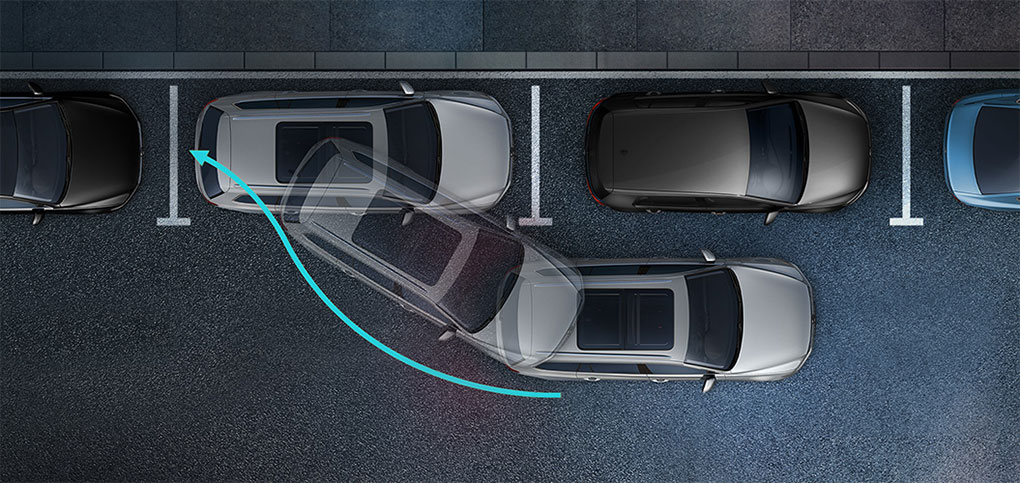
\includegraphics[width=0.9\textwidth]{images/auto-par.jpg}
\end{center}
\hfill Image Credit: Volkswagen


Wait\ldots autonomous vehicles is a different course\ldots

\end{frame}

 
%%%%%%%%%%%%%%%%%%%%%%%%%%%%%%%%%%%%%%%%%%%%%%%%%%%%%%%%%%%%%%%%%%%%%%%%%%%%%%%%
\begin{frame}
  \frametitle{Three Address Code}

  
  \begin{itemize}
    \item An intermediate code used by compilers
      for analysis and optimization.
    \vfill
    \item Statements represent one fundamental operation---we
      can consider each operation \structure{atomic}.
    \vfill
    \item Statements have the form:\\
      $\qquad result := operand_1\:operator\:operand_2$
    \vfill
    \item Useful for reasoning about data races,\\ and easier to read than assembly. \\
            \hspace*{1cm} (separates out memory reads/writes).
  \end{itemize}
  
\end{frame}
%%%%%%%%%%%%%%%%%%%%%%%%%%%%%%%%%%%%%%%%%%%%%%%%%%%%%%%%%%%%%%%%%%%%%%%%%%%%%%%%

%%%%%%%%%%%%%%%%%%%%%%%%%%%%%%%%%%%%%%%%%%%%%%%%%%%%%%%%%%%%%%%%%%%%%%%%%%%%%%%%
\begin{frame}
  \frametitle{GIMPLE}

  
  \begin{itemize}
    \item GIMPLE is the three address code used by {\tt gcc}.
    \vfill
    \item To see the GIMPLE representation of your code use the
      {\tt -fdump-tree-gimple} flag.
    \vfill
    \item To see all of the three address code generated by the compiler use
      {\tt -fdump-tree-all}. You'll probably just be interested in the
      optimized version.
    \vfill
    \item Use GIMPLE to reason about your code at a low level without
      having to read assembly.
  \end{itemize}
  
\end{frame}
%%%%%%%%%%%%%%%%%%%%%%%%%%%%%%%%%%%%%%%%%%%%%%%%%%%%%%%%%%%%%%%%%%%%%%%%%%%%%%%%

%%%%%%%%%%%%%%%%%%%%%%%%%%%%%%%%%%%%%%%%%%%%%%%%%%%%%%%%%%%%%%%%%%%%%%%%%%%%%%%%
\begin{frame}
  \frametitle{The {\tt restrict} Keyword}

   
   A feature available as of C99: ``The restrict type qualifier allows programs to
      be written so that translators can produce significantly faster
      executables.''
  \begin{itemize}
    \item {\tt gcc} 5+ support C11 or better by default.
  \end{itemize}
~\\
   {\tt restrict} means: you are promising the
      compiler that the pointer will never \structure{alias} (another pointer
      will not point to the same data) for the lifetime of the pointer.
  

\end{frame}
%%%%%%%%%%%%%%%%%%%%%%%%%%%%%%%%%%%%%%%%%%%%%%%%%%%%%%%%%%%%%%%%%%%%%%%%%%%%%%%%

\begin{frame}
\frametitle{Take the Vow}

\begin{center}
	
\includegraphics[width=0.5\textwidth]{images/solemnlyswear.jpg}
\end{center}


\end{frame}

%%%%%%%%%%%%%%%%%%%%%%%%%%%%%%%%%%%%%%%%%%%%%%%%%%%%%%%%%%%%%%%%%%%%%%%%%%%%%%%%
\begin{frame}[fragile]
  \frametitle{Example of {\tt restrict} (1)}

  
    Pointers declared with {\tt restrict} must
       never point to the same data.
~\\[1em]
    From Wikipedia:

  \begin{lstlisting}[language=C]
void updatePtrs(int* ptrA, int* ptrB, int* val) {
    *ptrA += *val;
    *ptrB += *val;
}
  \end{lstlisting}
 Would declaring all these pointers as
      {\tt restrict} generate better code?
  

\end{frame}
%%%%%%%%%%%%%%%%%%%%%%%%%%%%%%%%%%%%%%%%%%%%%%%%%%%%%%%%%%%%%%%%%%%%%%%%%%%%%%%%

%%%%%%%%%%%%%%%%%%%%%%%%%%%%%%%%%%%%%%%%%%%%%%%%%%%%%%%%%%%%%%%%%%%%%%%%%%%%%%%%
\begin{frame}[fragile]
  \frametitle{Example of {\tt restrict} (2)}

  
    Let's look at the GIMPLE:

  \begin{lstlisting}[language=C][numbers=left]
void updatePtrs(int* ptrA, int* ptrB, int* val) {
 D.1609 = *ptrA;
 D.1610 = *val;
 D.1611 = D.1609 + D.1610;
 *ptrA = D.1611;
 D.1612 = *ptrB;
 D.1610 = *val;
 D.1613 = D.1612 + D.1610;
 *ptrB = D.1613;
}
  \end{lstlisting}

  \begin{itemize}
    \item Could any operation be left out if all the pointers
      didn't overlap?
  \end{itemize}  
  

\end{frame}
%%%%%%%%%%%%%%%%%%%%%%%%%%%%%%%%%%%%%%%%%%%%%%%%%%%%%%%%%%%%%%%%%%%%%%%%%%%%%%%%

%%%%%%%%%%%%%%%%%%%%%%%%%%%%%%%%%%%%%%%%%%%%%%%%%%%%%%%%%%%%%%%%%%%%%%%%%%%%%%%%
\begin{frame}[fragile]
  \frametitle{Example of {\tt restrict} (3)}

  
  \begin{lstlisting}[language=C][numbers=left]
void updatePtrs(int* ptrA, int* ptrB, int* val) {
 D.1609 = *ptrA;
 D.1610 = *val;
 D.1611 = D.1609 + D.1610;
 *ptrA = D.1611;
 D.1612 = *ptrB;
 D.1610 = *val;
 D.1613 = D.1612 + D.1610;
 *ptrB = D.1613;
}
  \end{lstlisting}
  \begin{itemize}
    \item If {\tt ptrA} and {\tt val} are not equal, you don't have to
      reload the data on {\bf line 7}.
    \item Otherwise, you would: there might be a call\\{\tt ~~~~updatePtrs(\&x, \&y,
      \&x);}
  \end{itemize}
  
\end{frame}
%%%%%%%%%%%%%%%%%%%%%%%%%%%%%%%%%%%%%%%%%%%%%%%%%%%%%%%%%%%%%%%%%%%%%%%%%%%%%%%%

%%%%%%%%%%%%%%%%%%%%%%%%%%%%%%%%%%%%%%%%%%%%%%%%%%%%%%%%%%%%%%%%%%%%%%%%%%%%%%%%
\begin{frame}[fragile]
  \frametitle{Example of {\tt restrict} (4)}
  
  Hence, this markup allows optimization:
  \begin{lstlisting}[language=C]
void updatePtrs(int* restrict ptrA, 
                int* restrict ptrB,
                int* restrict val)
  \end{lstlisting}
  Note: you can get the optimization by just declaring {\tt ptrA} and
      {\tt val} as {\tt restrict}; {\tt ptrB} isn't needed for this optimization
  
\end{frame}
%%%%%%%%%%%%%%%%%%%%%%%%%%%%%%%%%%%%%%%%%%%%%%%%%%%%%%%%%%%%%%%%%%%%%%%%%%%%%%%%

%%%%%%%%%%%%%%%%%%%%%%%%%%%%%%%%%%%%%%%%%%%%%%%%%%%%%%%%%%%%%%%%%%%%%%%%%%%%%%%%
\begin{frame}[fragile]
  \frametitle{Summary of {\tt restrict}}

  
  \begin{itemize}
    \item Use {\tt restrict} whenever you know the pointer will not alias
      another pointer (also declared {\tt restrict})
  \end{itemize}

    It's hard for the compiler to infer pointer aliasing information;
    it's easier for you to specify it.\\[1em]

    $\Rightarrow$ compiler can better optimize your code (more perf!)\\[1em]
    
\end{frame}


\begin{frame}
\frametitle{Summary of {\tt restrict}}

\begin{center}
	
\includegraphics[width=0.4\textwidth]{images/i-lied.jpg}
\end{center}

    Caveat: don't lie to the compiler, or  you will get
      \alert{undefined behaviour}.\\[1em]

    Aside: {\tt restrict} is not the same as {\tt const}. {\tt const} data can still be
      changed through an alias.
  
\end{frame}
%%%%%%%%%%%%%%%%%%%%%%%%%%%%%%%%%%%%%%%%%%%%%%%%%%%%%%%%%%%%%%%%%%%%%%%%%%%%%%%%

%%%%%%%%%%%%%%%%%%%%%%%%%%%%%%%%%%%%%%%%%%%%%%%%%%%%%%%%%%%%%%%%%%%%%%%%%%%%%%%%
\begin{frame}[fragile]
  \frametitle{Automatic Parallelization of Example Code}


  Let's try automatic parallelization.
  \vfill
  Compiling with {\tt solarisstudio} and automatic parallelization yields
  the following:


{\scriptsize
  \begin{lstlisting}[language=C]
% solarisstudio-cc -O3 -xautopar -xloopinfo omp_vector.c 
"omp_vector.c", line 5: PARALLELIZED, and serial version generated                 
"omp_vector.c", line 15: not parallelized, call may be unsafe
  \end{lstlisting}
}

  How will this code compare to our manual efforts? \\
  (If you weren't in class, you'll have to try it yourself.)
  \vfill
  {\bf Note:} {\tt solarisstudio} generates two versions of the code, 
  and decides, at runtime, if the parallel code would be faster.


\end{frame}
%%%%%%%%%%%%%%%%%%%%%%%%%%%%%%%%%%%%%%%%%%%%%%%%%%%%%%%%%%%%%%%%%%%%%%%%%%%%%%%%

%%%%%%%%%%%%%%%%%%%%%%%%%%%%%%%%%%%%%%%%%%%%%%%%%%%%%%%%%%%%%%%%%%%%%%%%%%%%%%%%
\begin{frame}[fragile]
  \frametitle{Example Code to Parallelize}


  \begin{lstlisting}[language=C][numbers=left]
#include <stdlib.h>

void setup(double *vector, int length) {
    int i;
    for (i = 0; i < length; i++)
    {
        vector[i] += 1.0;
    }
}

int main()
{
    double *vector;
    vector = (double*) malloc(sizeof(double)*1024*1024);
    for (int i = 0; i < 1000; i++)
    {
        setup (vector, 1024*1024);
    }
    // if you don't read vector, compiler NOPs everything
    printf("%f\n", vector[0]);
}
  \end{lstlisting}

\end{frame}
%%%%%%%%%%%%%%%%%%%%%%%%%%%%%%%%%%%%%%%%%%%%%%%%%%%%%%%%%%%%%%%%%%%%%%%%%%%%%%%%

%%%%%%%%%%%%%%%%%%%%%%%%%%%%%%%%%%%%%%%%%%%%%%%%%%%%%%%%%%%%%%%%%%%%%%%%%%%%%%%%
\begin{frame}[fragile]
  \frametitle{Automatic Parallelization of Example Code}


  Let's try automatic parallelization.
  \vfill
  Compiling with {\tt solarisstudio} and automatic parallelization yields
  the following:


{\scriptsize
  \begin{lstlisting}[language=C]
% solarisstudio-cc -O3 -xautopar -xloopinfo omp_vector.c 
"omp_vector.c", line 5: PARALLELIZED, and serial version generated                 
"omp_vector.c", line 15: not parallelized, call may be unsafe
  \end{lstlisting}
}

  How will this code compare to our manual efforts? \\
  (If you weren't in class, you'll have to try it yourself.)
  \vfill
  {\bf Note:} {\tt solarisstudio} generates two versions of the code, 
  and decides, at runtime, if the parallel code would be faster.


\end{frame}
%%%%%%%%%%%%%%%%%%%%%%%%%%%%%%%%%%%%%%%%%%%%%%%%%%%%%%%%%%%%%%%%%%%%%%%%%%%%%%%%


%%%%%%%%%%%%%%%%%%%%%%%%%%%%%%%%%%%%%%%%%%%%%%%%%%%%%%%%%%%%%%%%%%%%%%%%%%%%%%%%
\begin{frame}
  \frametitle{Autoparallelization implementation: OpenMP}

\begin{center}
	
\includegraphics[width=0.4\textwidth]{images/openmp.png}
\end{center}

  Under the hood, most parallelization frameworks use {\tt OpenMP},
      which we'll see next lecture.
      
  For now: you can control the number of threads with the
      {\tt OMP\_NUM\_THREADS} environment variable.

\end{frame}
%%%%%%%%%%%%%%%%%%%%%%%%%%%%%%%%%%%%%%%%%%%%%%%%%%%%%%%%%%%%%%%%%%%%%%%%%%%%%%%%

%%%%%%%%%%%%%%%%%%%%%%%%%%%%%%%%%%%%%%%%%%%%%%%%%%%%%%%%%%%%%%%%%%%%%%%%%%%%%%%%
\begin{frame}[fragile]
  \frametitle{Automatic Parallelization in {\tt gcc}}


  {\tt gcc} (since 4.3) can also auto-parallelize loops via Graphite. \\[1em]
  Parallelization has been getting better, \\ \qquad but not super well-maintained.\\[1em]
  I think {\tt gcc} can insert a runtime check of loop iteration count.\\[2em]
  
\begin{center}
	
\includegraphics[width=0.4\textwidth]{images/dandc.jpg}
\end{center}

\end{frame}

\begin{frame}[fragile]
  \frametitle{Automatic Parallelization in {\tt gcc}}  
  Magic incantation:\\
  \qquad {\tt gcc -O2 -floop-parallelize-all }\\
  \qquad \qquad {\tt -ftree-parallelize-loops=4 -fopt-info}\\[1em]
  {\tt -floop-parallelize-all:} parallelize all the things\\
  {\tt -ftree-parallelize-loops=N:} use {\tt N} threads\\[1em]

  {\bf Note:} {\tt gcc} uses {\tt OpenMP} but overrides
  {\tt OMP\_NUM\_THREADS} with {\tt N} above.


\end{frame}
%%%%%%%%%%%%%%%%%%%%%%%%%%%%%%%%%%%%%%%%%%%%%%%%%%%%%%%%%%%%%%%%%%%%%%%%%%%%%%%%

%%%%%%%%%%%%%%%%%%%%%%%%%%%%%%%%%%%%%%%%%%%%%%%%%%%%%%%%%%%%%%%%%%%%%%%%%%%%%%%%
\begin{frame}[fragile]
  \frametitle{Sample {\tt -fopt-info} output}

\begin{verbatim}
$ gcc L11-omp_vector.c -O2 \
 -floop-parallelize-all -ftree-parallelize-loops=4 -fopt-info 
L11-omp_vector.c:14:3: note: parallelizing inner loop 1
L11-omp_vector.c:23:3: note: loop nest optimized
L11-omp_vector.c:15:15: note: parallelizing inner loop 4

line 14: for (i = 0; i < length; i++) {
line 15: vector[i] += 1.0;
line 23: for (int i = 0; i < 1000; i++) {
\end{verbatim}


\end{frame}
%%%%%%%%%%%%%%%%%%%%%%%%%%%%%%%%%%%%%%%%%%%%%%%%%%%%%%%%%%%%%%%%%%%%%%%%%%%%%%%%

%%%%%%%%%%%%%%%%%%%%%%%%%%%%%%%%%%%%%%%%%%%%%%%%%%%%%%%%%%%%%%%%%%%%%%%%%%%%%%%%
\begin{frame}[fragile]
  \frametitle{Understanding Automatic Parallelization in {\tt gcc}}


  Want to better understand?\\
  Look at the assembly code to see the parallelizations\\
  (obviously, impractical for a large project).\\[-7em]
\begin{verbatim}
$ gcc -std=c99 -O3 -ftree-parallelize-loops=4 \
    omp_vector_gcc.c -S -o omp_vector_gcc_auto.s
\end{verbatim}
  [Or, you can use {\tt objdump} on files compiled with {\tt -g}.]
  
\end{frame}
%%%%%%%%%%%%%%%%%%%%%%%%%%%%%%%%%%%%%%%%%%%%%%%%%%%%%%%%%%%%%%%%%%%%%%%%%%%%%%%%

%%%%%%%%%%%%%%%%%%%%%%%%%%%%%%%%%%%%%%%%%%%%%%%%%%%%%%%%%%%%%%%%%%%%%%%%%%%%%%%%
\begin{frame}[fragile]

\begin{center}
	
\includegraphics[width=0.3\textwidth]{images/microscope.jpeg}
\end{center}

  \frametitle{{\tt gcc} assembly output}
  Older gcc generated a {\tt .s} file with:
  \begin{lstlisting}[language=C]
call    GOMP_parallel_start
leaq    80(%rsp), %rdi
call    setup._loopfn.0
call    GOMP_parallel_end
  \end{lstlisting}
  \vfill
  {\bf Note:} {\tt gcc} also parallelizes {\tt main.\_loopfn.2} and
  {\tt main.\_loopfn.3}, although it looks like it serves little purpose.


\end{frame}
%%%%%%%%%%%%%%%%%%%%%%%%%%%%%%%%%%%%%%%%%%%%%%%%%%%%%%%%%%%%%%%%%%%%%%%%%%%%%%%%

%%%%%%%%%%%%%%%%%%%%%%%%%%%%%%%%%%%%%%%%%%%%%%%%%%%%%%%%%%%%%%%%%%%%%%%%%%%%%%%%
\begin{frame}[fragile]
  \frametitle{Loops gcc Can Handle}


  Single loop:
  \begin{lstlisting}[language=C]
for (i = 0; i < 1000; i++)
    x[i] = i + 3;
  \end{lstlisting}
  \vfill
  Nested loops with simple dependency:
  \begin{lstlisting}[language=C]
for (i = 0; i < 100; i++)
    for (j = 0; j < 100; j++)
        X[i][j] = X[i][j] + Y[i-1][j];
  \end{lstlisting}
  \vfill
  Single loop with not-very-simple dependency:
  \begin{lstlisting}[language=C]
for (i = 0; i < 10; i++)
    X[2*i+1] = X[2*i];
  \end{lstlisting}

\end{frame}
%%%%%%%%%%%%%%%%%%%%%%%%%%%%%%%%%%%%%%%%%%%%%%%%%%%%%%%%%%%%%%%%%%%%%%%%%%%%%%%%

%%%%%%%%%%%%%%%%%%%%%%%%%%%%%%%%%%%%%%%%%%%%%%%%%%%%%%%%%%%%%%%%%%%%%%%%%%%%%%%%
\begin{frame}[fragile]
  \frametitle{More Loops gcc Can Handle}


  Single loop with if statement:
  \begin{lstlisting}[language=C]
for (j = 0; j <= 10; j++)
    if (j > 5) X[i] = i + 3;
  \end{lstlisting}
  \vfill
  Triangle loop:
  \begin{lstlisting}[language=C]
for (i = 0; i < 100; i++)
    for (j = i; j < 100; j++)
        X[i][j] = 5;
  \end{lstlisting}
  \vfill
  Examples from: \url{http://gcc.gnu.org/wiki/AutoparRelated}

\end{frame}
%%%%%%%%%%%%%%%%%%%%%%%%%%%%%%%%%%%%%%%%%%%%%%%%%%%%%%%%%%%%%%%%%%%%%%%%%%%%%%%%

%%%%%%%%%%%%%%%%%%%%%%%%%%%%%%%%%%%%%%%%%%%%%%%%%%%%%%%%%%%%%%%%%%%%%%%%%%%%%%%%
\begin{frame}
  \frametitle{Summary of Conditions for Automatic Parallelization}


  From Chapter 10 of
  Oracle's \emph{Fortran Programming Guide}
  \footnote{\scriptsize \url{http://download.oracle.com/docs/cd/E19205-01/819-5262/index.html}}
  translated to C, a loop must:

  \begin{itemize}
    \item have a recognized loop style, e.g., {\tt for} loops with
      bounds that don't vary per-iteration;
    \item have no dependencies between data accessed in loop bodies for
      each iteration;
    \item not conditionally change scalar variables read after the loop
      terminates, or change any scalar variable across iterations; and
    \item have enough work in the loop body to make parallelization profitable.
  \end{itemize}

\end{frame}
%%%%%%%%%%%%%%%%%%%%%%%%%%%%%%%%%%%%%%%%%%%%%%%%%%%%%%%%%%%%%%%%%%%%%%%%%%%%%%%%


\begin{frame}
\frametitle{Let's Race}

\begin{center}
	
\includegraphics[width=\textwidth]{images/imbatman.jpg}
\end{center}


\end{frame}


%%%%%%%%%%%%%%%%%%%%%%%%%%%%%%%%%%%%%%%%%%%%%%%%%%%%%%%%%%%%%%%%%%%%%%%%%%%%%%%%
\begin{frame}[fragile]
  \frametitle{Example Code to Parallelize (once more)}


  \begin{lstlisting}[language=C][numbers=left]
#include <stdlib.h>

void setup(double *vector, int length) {
    int i;
    for (i = 0; i < length; i++)
    {
        vector[i] += 1.0;
    }
}

int main()
{
    double *vector;
    vector = (double*) malloc(sizeof(double)*1024*1024);
    for (int i = 0; i < 1000; i++)
    {
        setup (vector, 1024*1024);
    }
    // if you don't read vector, compiler NOPs everything
    printf("%f\n", vector[0]);
}
  \end{lstlisting}

\end{frame}
%%%%%%%%%%%%%%%%%%%%%%%%%%%%%%%%%%%%%%%%%%%%%%%%%%%%%%%%%%%%%%%%%%%%%%%%%%%%%%%%



%%%%%%%%%%%%%%%%%%%%%%%%%%%%%%%%%%%%%%%%%%%%%%%%%%%%%%%%%%%%%%%%%%%%%%%%%%%%%%%%
\begin{frame}
  \frametitle{Manually Parallelizing the Example Code}


  What can we do to parallelize this code?
  \vfill
  {\bf Option 1:} \uncover<2->{ horizontal~ \qquad \begin{minipage}{7em} --- --- --- ---\\[-.8em] --- --- --- ---\\[-.8em] --- --- --- --- \end{minipage}}

  \begin{itemize}
    \item<2-> Create 4 threads; each thread does 1000 iterations on its own sub-array.
  \end{itemize}

  {\bf Option 2:} \uncover<3->{ bad horizontal~~ \begin{minipage}{7em} --- --- --- ---\\[-.8em] --- --- --- ---\\[-.8em] --- --- --- --- \end{minipage}}

  \begin{itemize}
    \item<3-> 1000 times, create 4 threads which each operate once on the sub-array.
  \end{itemize}

  {\bf Option 3:} \uncover<4->{~~vertical $ \quad \: \qquad \mid \mid \mid\mid \:\: \mid \mid \mid \mid \:\: \mid \mid \mid \mid\:\: \mid \mid \mid \mid$}
  \begin{itemize}
    \item<4-> Create 4 threads; for each element, the owning thread does 1000 iterations on that element.
  \end{itemize}

\end{frame}
%%%%%%%%%%%%%%%%%%%%%%%%%%%%%%%%%%%%%%%%%%%%%%%%%%%%%%%%%%%%%%%%%%%%%%%%%%%%%%%%

%%%%%%%%%%%%%%%%%%%%%%%%%%%%%%%%%%%%%%%%%%%%%%%%%%%%%%%%%%%%%%%%%%%%%%%%%%%%%%%%
\begin{frame}
  \frametitle{Manual Parallelization Demo}

  Methodology: compiling with {\tt solarisstudio}, \\ flags {\tt -O3 -lpthread}.\\[1em]

  Which manual option performs better?


\end{frame}
%%%%%%%%%%%%%%%%%%%%%%%%%%%%%%%%%%%%%%%%%%%%%%%%%%%%%%%%%%%%%%%%%%%%%%%%%%%%%%%%


%%%%%%%%%%%%%%%%%%%%%%%%%%%%%%%%%%%%%%%%%%%%%%%%%%%%%%%%%%%%%%%%%%%%%%%%%%%%%%%%
\begin{frame}[fragile]
  \frametitle{Comparing Parallelization Results}


How does autoparallelization compare to manual parallelization?
   \begin{itemize}
     \item<2-> Relative ordering: {\bf Option 3} \textgreater{} Automatic
       \textgreater{} {\bf Option 1}
     \item<2-> Automatic parallelization of {\bf Option 1} was better than
       manual, why?
     \item<3-> Manual {\bf Option 3} performed better, even though both used the
       same number of threads, why?
   \end{itemize}


\end{frame}
%%%%%%%%%%%%%%%%%%%%%%%%%%%%%%%%%%%%%%%%%%%%%%%%%%%%%%%%%%%%%%%%%%%%%%%%%%%%%%%%

%%%%%%%%%%%%%%%%%%%%%%%%%%%%%%%%%%%%%%%%%%%%%%%%%%%%%%%%%%%%%%%%%%%%%%%%%%%%%%%%
\begin{frame}[containsverbatim]
  \frametitle{Lingering Questions about Runtimes}

  
    What happened here?\\[1em]
  
    \begin{tabular}{ll}
      \begin{minipage}{5em} --- --- --- ---\\[-.8em] --- --- --- ---\\[-.8em] --- --- --- --- \end{minipage}& horizontal good: \\
      & \qquad create 4 threads to do 1000 iterations on sub-arrays.\\
      \begin{minipage}{5em} --- --- --- ---\\[-.8em] --- --- --- ---\\[-.8em] --- --- --- --- \end{minipage}& horizontal bad: \\
      & \qquad 1000 times, create 4 threads to iterate on sub-array. \\
      $ \mid \mid \mid\mid \: \mid \mid \mid \mid \: \mid \mid \mid \mid\: \mid \mid \mid \mid$& vertical:\\
      & \qquad create 4 threads, handle 1 element at a time.\\[1em]
    \end{tabular}
    
      
      In 2015, {\tt perf stat -r 5} gave following task-clocks (in seconds):\\[1em]

      \begin{center}
      \begin{tabular}{lrrrr}
        & H good & H bad & V & auto \\
        gcc, no opt & 2.794 & 2.953 & 2.799\\
        gcc, -O3 & 0.588 & 1.490 & 0.980\\
        solaris, no opt & 3.175 & 3.291 & 2.966 \\
        solaris, -xO4 & 0.494 & 1.453 & 2.739 & 0.688\\
      \end{tabular}
      \end{center}
  
\end{frame}
%%%%%%%%%%%%%%%%%%%%%%%%%%%%%%%%%%%%%%%%%%%%%%%%%%%%%%%%%%%%%%%%%%%%%%%%%%%%%%%%

%%%%%%%%%%%%%%%%%%%%%%%%%%%%%%%%%%%%%%%%%%%%%%%%%%%%%%%%%%%%%%%%%%%%%%%%%%%%%%%%
\begin{frame}[containsverbatim]
  \frametitle{Runtimes---Why?}

  
    Observations:\\[1em]
    \begin{itemize}
    \item Good runs had 5 to 7 cpu-migrations; bad had 4000.
    \item \# cycles varied from 2B to 9.7B (no opt).\\
    \item Branch misses varied from 8k to 208k.
    \end{itemize}
  
    

    
%%     gcc plain, bad: 4,004 cpu-migrations; 5.2B cycles; 75\% frontend cycles idle; 1B branches; 167k branch misses
%% gcc -O3, bad: 4,003 cpu-migrations; 4.2B cycles; 80\% frontend cycles idle; 466k branches; 208k branch misses
%% gcc plain, good: 5 cpu-migrations; 9.6B cycles; 39\% frontend cycles idle; 1B branches; 13k branch misses
%% gcc -O3, good: 7 cpu-migrations; 2B cycles; 49\% frontend cycles idle; 525k branches; 8k branch misses

%% gcc plain, V: 5 cpu-migrations; 9.7B cycles; 44\% frontend cycles idle; 1B branches; 1M branch misses
%% gcc -O3, V: 7 cpu-migrations; 3.3B cycles; 69\% frontend cycles idle; 1B branches; 1M branch misses

%% solaris auto: 0.688s; 3 cpu-migrations; 2.4B cycles; 72\% frontend cycles idle; 134M branches; 30k branch misses
        
    
\end{frame}
%%%%%%%%%%%%%%%%%%%%%%%%%%%%%%%%%%%%%%%%%%%%%%%%%%%%%%%%%%%%%%%%%%%%%%%%%%%%%%%%


%%%%%%%%%%%%%%%%%%%%%%%%%%%%%%%%%%%%%%%%%%%%%%%%%%%%%%%%%%%%%%%%%%%%%%%%%%%%%%%%
\begin{frame}[fragile]
  \frametitle{Case Study 2: Multiplying a Matrix by a Vector}


Let's see how automatic parallelization does on a more complicated
program (could we parallelize this?):

  \begin{lstlisting}[language=C][numbers=left]
void matVec (double **mat, double *vec, double *out,
             int *row, int *col) 
{
  int i, j;
  for (i = 0; i < *row; i++)
  {
    out[i] = 0;
    for (j = 0; j < *col; j++)
    {
      out[i] += mat[i][j] * vec[j];
    }
  }
}
  \end{lstlisting}


  \begin{center}
    Reminder:
    \begin{math}
      \begin{bmatrix} 1 & 2 & 3 \\ 4 & 5 & 6\end{bmatrix}
      \begin{bmatrix} 1 \\ 2 \\ 3 \end{bmatrix}
      =
      \begin{bmatrix} 14 \\ 32 \end{bmatrix}
    \end{math}
  \end{center}

\end{frame}
%%%%%%%%%%%%%%%%%%%%%%%%%%%%%%%%%%%%%%%%%%%%%%%%%%%%%%%%%%%%%%%%%%%%%%%%%%%%%%%%

%%%%%%%%%%%%%%%%%%%%%%%%%%%%%%%%%%%%%%%%%%%%%%%%%%%%%%%%%%%%%%%%%%%%%%%%%%%%%%%%
\begin{frame}[fragile]
  \frametitle{Case Study: Automatic Parallelization, Attempt 1}

  
  Well, based on our knowledge, we could parallelize the outer loop.\\[1em]
  Let's see what {\tt solarisstudio} will do for us\ldots
  

  \begin{lstlisting}[language=C]
% solarisstudio-cc -xautopar -xloopinfo -O3 -c fploop.c
"fploop.c", line 5: not parallelized, not a recognized for loop
"fploop.c", line 8: not parallelized, not a recognized for loop
  \end{lstlisting}

  
  \ldots it refuses to do anything, guesses?
  

\end{frame}
%%%%%%%%%%%%%%%%%%%%%%%%%%%%%%%%%%%%%%%%%%%%%%%%%%%%%%%%%%%%%%%%%%%%%%%%%%%%%%%%

%%%%%%%%%%%%%%%%%%%%%%%%%%%%%%%%%%%%%%%%%%%%%%%%%%%%%%%%%%%%%%%%%%%%%%%%%%%%%%%%
\begin{frame}[fragile]
  \frametitle{Case Study: Automatic Parallelization, Attempt 2}


  \begin{itemize}
    \item The loop bounds are not constant, since one of the variables may alias
      {\tt row} or {\tt col}, even though {\tt int $\neq$ double}.
  \end{itemize}
~\\[1em]

  So, let's add {\tt restrict} to {\tt row} and {\tt col} and see what
  happens\ldots

  \begin{lstlisting}[language=C]
% solarisstudio-cc -O3 -xautopar -xloopinfo -c fploop.c
"fploop.c", line 5: not parallelized, unsafe dependence
"fploop.c", line 8: not parallelized, unsafe dependence
  \end{lstlisting}

  Now it recognizes the loop, but still won't parallelize it. Why?


\end{frame}
%%%%%%%%%%%%%%%%%%%%%%%%%%%%%%%%%%%%%%%%%%%%%%%%%%%%%%%%%%%%%%%%%%%%%%%%%%%%%%%%

%%%%%%%%%%%%%%%%%%%%%%%%%%%%%%%%%%%%%%%%%%%%%%%%%%%%%%%%%%%%%%%%%%%%%%%%%%%%%%%%
\begin{frame}[fragile]
  \frametitle{Case Study: Automatic Parallelization, Attempt 3}


  \begin{itemize}
    \item {\tt out} might alias {\tt mat} or {\tt vec}, which would make this
      unsafe
  \end{itemize}

  Let's add another {\tt restrict} to {\tt out}:

  \begin{lstlisting}[language=C]
% solarisstudio-cc -O3 -xautopar -xloopinfo -c fploop.c
"fploop.c", line 5: PARALLELIZED, and serial version
  generated
"fploop.c", line 8: not parallelized, unsafe dependence
  \end{lstlisting}

  Now, we can get the outer loop to parallelize.
  
  \begin{itemize}
    \item Parallelizing the outer loop is almost always better than inner loops,
      and usually it's a waste to do both, so we're done.
  \end{itemize}

  {\bf Note:} We can parallelize the inner loop as well (it's similar to
the assignment). We'll see that {\tt solarisstudio} can do it automatically.


\end{frame}
%%%%%%%%%%%%%%%%%%%%%%%%%%%%%%%%%%%%%%%%%%%%%%%%%%%%%%%%%%%%%%%%%%%%%%%%%%%%%%%%


%%%%%%%%%%%%%%%%%%%%%%%%%%%%%%%%%%%%%%%%%%%%%%%%%%%%%%%%%%%%%%%%%%%%%%%%%%%%%%%%
\begin{frame}
  \frametitle{Reductions}

\begin{center}
	
\includegraphics[width=0.5\textwidth]{images/highlander.jpeg}
\end{center}

 Reductions combine input data into a smaller (summary) set.

\end{frame}


\begin{frame}[fragile]
\frametitle{Reduction Example}

Simplest instance: computing the sum of an array.
 
  Consider the following code:

  \begin{lstlisting}[language=C]
double sum (double *array, int length)
{
  double total = 0;

  for (int i = 0; i < length; i++)
    total += array[i];
  return total;
}
  \end{lstlisting}

  Can we parallelize this? 

\end{frame}
%%%%%%%%%%%%%%%%%%%%%%%%%%%%%%%%%%%%%%%%%%%%%%%%%%%%%%%%%%%%%%%%%%%%%%%%%%%%%%%%

%%%%%%%%%%%%%%%%%%%%%%%%%%%%%%%%%%%%%%%%%%%%%%%%%%%%%%%%%%%%%%%%%%%%%%%%%%%%%%%%
\begin{frame}[fragile]
  \frametitle{Reduction Problems}


  Barriers to parallelization:
  \begin{enumerate}
    \item value of {\tt total} depends on previous
      iterations;
    \item addition is actually non-associative for floating-point values
      \\ (is this a problem?)
  \end{enumerate}
  ~\\[1em]
  \begin{center}
    Recall that ``associative'' means: 
     \[a + (b + c) = (a + b) + c.\]
  \end{center}
	 In this case, the program probably isn't sensitive to rounding,
      but you should always consider if an operation is associative.

\end{frame}
%%%%%%%%%%%%%%%%%%%%%%%%%%%%%%%%%%%%%%%%%%%%%%%%%%%%%%%%%%%%%%%%%%%%%%%%%%%%%%%%

%%%%%%%%%%%%%%%%%%%%%%%%%%%%%%%%%%%%%%%%%%%%%%%%%%%%%%%%%%%%%%%%%%%%%%%%%%%%%%%%
\begin{frame}[fragile]
  \frametitle{Automatic Parallelization via Reduction}


  If we compile the program with {\tt solarisstudio} and add the flag
  {\tt -xreduction}, it will parallelize the code:


  \begin{lstlisting}[language=C]
% solarisstudio-cc -xautopar -xloopinfo -xreduction -O3 -c sum.c 
"sum.c", line 5: PARALLELIZED, reduction, and serial version
  generated
  \end{lstlisting}
~\\[1em]


  {\bf Note:} If we try to do the reduction on {\tt fploop.c} with {\tt restrict}s added, we'll get the following:


  \begin{lstlisting}[language=C]
% solarisstudio-cc -O3 -xautopar -xloopinfo  -xreduction -c fploop.c
"fploop.c", line 5: PARALLELIZED, and serial version generated
"fploop.c", line 8: not parallelized, not profitable
  \end{lstlisting}

\end{frame}
%%%%%%%%%%%%%%%%%%%%%%%%%%%%%%%%%%%%%%%%%%%%%%%%%%%%%%%%%%%%%%%%%%%%%%%%%%%%%%%%

%%%%%%%%%%%%%%%%%%%%%%%%%%%%%%%%%%%%%%%%%%%%%%%%%%%%%%%%%%%%%%%%%%%%%%%%%%%%%%%%
\begin{frame}
  \frametitle{Dealing with Function Calls}

  
  \begin{itemize}
    \item A general function could have arbitary side effects.
    \item Production compilers tend to avoid parallelizing any loops with
      function calls.
  \end{itemize}
~\\[1em]

  Some built-in functions, like {\tt sin()}, are ``pure'', have no side
  effects, and are safe to parallelize.
~\\[1em]
  {\bf Note:} this is why functional languages are nice for parallel
  programming: impurity is visible in type signatures.

\end{frame}
%%%%%%%%%%%%%%%%%%%%%%%%%%%%%%%%%%%%%%%%%%%%%%%%%%%%%%%%%%%%%%%%%%%%%%%%%%%%%%%%

%%%%%%%%%%%%%%%%%%%%%%%%%%%%%%%%%%%%%%%%%%%%%%%%%%%%%%%%%%%%%%%%%%%%%%%%%%%%%%%%
\begin{frame}
  \frametitle{Dealing with Function Calls in {\tt solarisstudio}}

  
  \begin{itemize}
    \item For {\tt solarisstudio} you can use the {\tt -xbuiltin} flag to make
      the compiler use its whitelist of ``pure'' functions.
    \item The compiler can then parallelize a loop which uses {\tt sin()}
      (you shouldn't replace built-in functions with your own if you use this
      option).
  \end{itemize}
  \vfill
  Other options which may work:
  
  \begin{enumerate}
    \item Crank up the optimization level ({\tt -xO4}).
    \item Explicitly tell the compiler to inline certain functions ({\tt
      -xinline=}, or use the {\tt inline} keyword).
  \end{enumerate}

\end{frame}
%%%%%%%%%%%%%%%%%%%%%%%%%%%%%%%%%%%%%%%%%%%%%%%%%%%%%%%%%%%%%%%%%%%%%%%%%%%%%%%%

%%%%%%%%%%%%%%%%%%%%%%%%%%%%%%%%%%%%%%%%%%%%%%%%%%%%%%%%%%%%%%%%%%%%%%%%%%%%%%%%
\begin{frame}
  \frametitle{Summary of Automatic Parallelization}

  
To help the compiler, we can:
\begin{itemize}
\item use {\tt restrict} (make a {\tt restrict}ed copy); and,
\item make sure that loop bounds are constant (temporary
variables). 
\end{itemize}
~\\
Some compilers automatically create different versions
for the alias-free case and the (parallelized) aliased case.\\[1em]

At runtime, the program runs the aliased case if correct.

\end{frame}
%%%%%%%%%%%%%%%%%%%%%%%%%%%%%%%%%%%%%%%%%%%%%%%%%%%%%%%%%%%%%%%%%%%%%%%%%%%%%%%%


\end{document}

